% This is samplepaper.tex, a sample chapter demonstrating the
% LLNCS macro package for Springer Computer Science proceedings;
% Version 2.20 of 2017/10/04
%
%\documentclass[runningheads]{llncs}
%
\documentclass{llncs}

\usepackage{graphicx}
\usepackage{float}
\floatstyle{plaintop}
\restylefloat{table}
% Used for displaying a sample figure. If possible, figure files should
% be included in EPS format.
%
% If you use the hyperref package, please uncomment the following line
% to display URLs in blue roman font according to Springer's eBook style:
% \renewcommand\UrlFont{\color{blue}\rmfamily}
% \usepackage[autocite=superscript, hyperref=true, sorting=nty, backref=true, backend=biber, style=apa, citestyle=authoryear]{biblatex}
\usepackage[spanish,es-tabla]{babel}
% \addbibresource{bib.bib}

\begin{document}
%
\title{Sistema de Recolección y Procesamiento de Datos para Estudios de Tránsito}
%
%\titlerunning{Abbreviated paper title}
% If the paper title is too long for the running head, you can set
% an abbreviated paper title here
%
 \author{Héctor Rodríguez Rangel$^{1}$,
 Rafael Imperial Rojo$^{1}$ Luis Alberto Morales Rosales$^{2}$, Sofía Isabel Fernández Gregorio$^{3}$ y Abraham Efraím Rodríguez Mata$^{4}$}
% %
 \authorrunning{Héctor et al.}
 % First names are abbreviated in the running head.
% % If there are more than two authors, 'et al.' is used.
% %
 \institute{$^{1}$Tecnológico Nacional de México, Campus Culiacán,
 \email{hector.rr@culiacan.tecnm.mx} \\
 $^{2}$Conacyt-Universidad Michoacana de San Nicolás de Hidalgo \\
 $^{3}$Instituto Tecnológico Superior de Martínez de la Torre\\
 $^{4}$Tecnólogico Nacional de México, Campus Chihuahua \\
 }
% %
\maketitle              % typeset the header of the contribution
%
\begin{abstract}
La movilidad urbana se incremento con el uso de automóviles, lo que origino también un aumento de accidentes de tránsito. Para estudiar este fenómeno se requiere de estudios (ET) de tránsito. Con el uso de inteligencia artificial (IA) es posible realizarlos sin modificar en gran medida la infraestructura urbana. Para el diseño de soluciones basadas en IA es necesario generar bases de datos que proporcionen información confiable para la calibración y desarrollo de soluciones que permitan realizar ET de manera automatizada. En este trabajo se presenta un sistema para generar un conjunto de datos a partir de vídeos tomados en un punto de observación. 

\keywords{Base de Datos \and Velocidad vehicular \and Visión Artificial.}
\end{abstract}
%
%
%
\section{Introducción}
El uso de automóviles es esencial en nuestra vida cotidiana. Según la organización Association for Safe International Road Travel (ASIRT), cada año mueren más de 1,3 millones de personas en accidentes de tráfico, y entre 20 y 50 millones más resultan heridos o incapacitados (\cite{1}).
En los accidentes viales, el exceso de velocidad es el factor más mortífero por lo que los estudios de tránsito proporcionan el principal suministro de información para detectar las posibles causas. El enfoque tradicional para realizar estudios de tránsito está influenciado por el uso de equipo especial.
Uno de los sensores que no requiere modificaciones en la infraestructura de una ciudad son las cámaras de videovigilancia proporcionando información en tiempo real. Al analizar los datos provenientes de cámaras es posible estimar atributos del flujo de tráfico, detectar congestión, accidentes y observar el comportamiento de los conductores  entre otros factores (\cite{Yang2019Vehicle}). 
La inteligencia artificial (IA) está revolucionando la sociedad moderna. Los investigadores y desarrolladores tanto de la industria automotriz como de seguridad vial están desarrollando activamente enfoques de conducción autónoma y monitoreo basados en el aprendizaje profundo. Sin embargo, antes de que la red neuronal llegue al vehículo de producción, primero requiere una evaluación de seguridad funcional rigurosa y la construcción de base de datos para poder entrenar dichas redes neuronales. En \cite{jjj} se describe las posibilidades y desafíos de integrar el aprendizaje profundo en vehículos autónomos y se estudian la creación de base de datos para el entrenamiento de dichas redes neuronales. \\
En este trabajo se presenta un sistema para generar un conjunto de datos a partir de vídeos tomados en un punto de observación de una vía carretera. La principal característica de estos vídeos es que no son tomados paralelamente a la vista de la cámara. Con la creación de este sistema podemos ayudar a desarrollar diferentes conjuntos de datos con el propósito de inferir la velocidad de objetos y extraer las características que el usuario considere como las más importantes. Por otro lado, el desarrollo de soluciones para la generación automática de estudios de tránsito requieren de bases de datos que recopilen diferentes condiciones para observar comportamientos y calibrar sus resultados. En el caso del estudio del flujo vehicular mexicano, no existen bases de datos públicas confiables que ayuden a esta labor. 

\section{Metodología}
Este trabajo está enfocado en la generación de la información del flujo vehicular de una vialidad a partir de secuencias de vídeo. Al investigar, no se encontró con un dataset (conjunto de datos) acorde a las necesidades del proyecto, por lo cual se decidió crear uno que se adapte.
La metodología para la extracción de estas características se describe en el diagrama de flujo de la Figura \ref{img:FlowSystem} la cual cuenta con 4 etapas: 1) Toma de muestras, 2) Limpieza de muestras, 3) Extracción de información, 4) Validación de la información, estas se describen a continuación:  

\begin{figure}[H]
    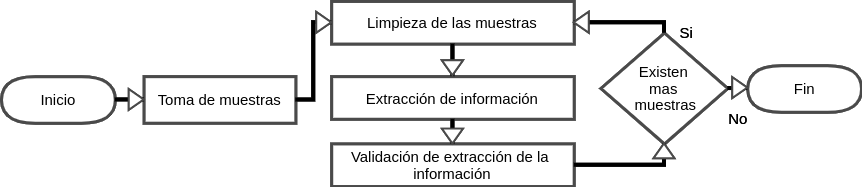
\includegraphics[width=0.8
    \textwidth]{imgs/FlowSystem2.png}
    \centering
    \caption{Diagrama de flujo metodología implementada.}
    \label{img:FlowSystem}
\end{figure}

\renewcommand{\labelitemi}{$-$}
\renewcommand{\labelitemii}{$\cdot$}
\begin{itemize}
    \item \textit{Toma de muestras.}  Se requirieron dos dispositivos para extraer el conjunto de datos. Los dispositivos son el radar Bushnell con una precisión de +/- 1.6 kilómetros por hora y una cámara de vídeo, para este caso se utilizó la cámara de teléfono inteligente configurados a 60 FPS y una resolución de Full HD (1920 x 1080 píxeles). Se posiciona la cámara de forma que los vehículos no pasen paralelamente a la vista de la cámara para que el cálculo no sea considerado como tomado en un plano 2D.  
    \item \textit{Limpieza de los muestras.} El radar no está integrado con el sistema de seguimiento. Se realiza la unión manual de la velocidad proporcionada por el radar y la información obtenida. Se requiere una inspección visual de las muestras tomadas, lo primero es identificar los puntos en $x$ que nos servirán como referencia para tomarlos como entrada y salida de los vehículos. Usando como referencia nuestro punto de salida, identificaremos los vehículos a los que se les tomo la velocidad y se anota el segundo en que pasa. Para esto se utiliza un archivo CSV, el cual cuenta con 2 campos:
     
        \begin{itemize}
            \item El segundo en que el objeto pasa por el punto de salida.
            \item La velocidad del objeto.
        \end{itemize}
        
    \item \textit{Extracción de información.} Para la generación del conjunto de datos se extraen las características principales del vídeo. Para el sistema presentado estas características son las siguientes:
\begin{itemize}
    \item Ángulo de salida: A partir del punto de entrada hasta el punto de salida.
    \item Distancia de salida: Distancia del punto de entrada hasta el de salida.
    \item Área de entrada: Área del vehículo en píxeles en el punto de entrada.
    \item Área de salida: Área del vehículo en píxeles en el punto de salida.
    \item FPS: Fotogramas por segundo del vídeo.
    \item Tiempo: Tiempo del punto entrada al de salida.
    \item Velocidad: Velocidad detectada por el radar.
    \item Identificador: Correspondiente a una imagen generada.
\end{itemize}
El proceso completo realizado por el sistema, comienza ejecutándolo dando como entrada el archivo CSV con las velocidades y los límites configurados previamente. Se decodifica el vídeo utilizando la biblioteca OpenCV la cual examina fotograma por fotograma, e identifica los vehículos con la red neuronal YOLO (\cite{YOLO}) esta se encarga de reconocer múltiples objetos en una sola predicción. Detectados todos los objetos dibuja la caja correspondiente a cada uno de ellos. El seguimiento se realiza por medio del filtro Kalman (\cite{welch1995introduction}) el cual determina su ubicación en el próximo fotograma. El sistema se encarga de guardar todas las ubicaciones de los vehículos en el transcurso del tiempo, con lo cual se traza todo el trayecto que han tenido cada uno de ellos, así como calcular la recta que corresponde a cada trayectoria. La Figura \ref{img:Tracking} muestra un vehículo detectado en un recuadro blanco, y un par de líneas amarilla y roja que corresponden al seguimiento y a la recta calculada a partir del seguimiento.
\begin{figure}[H]
    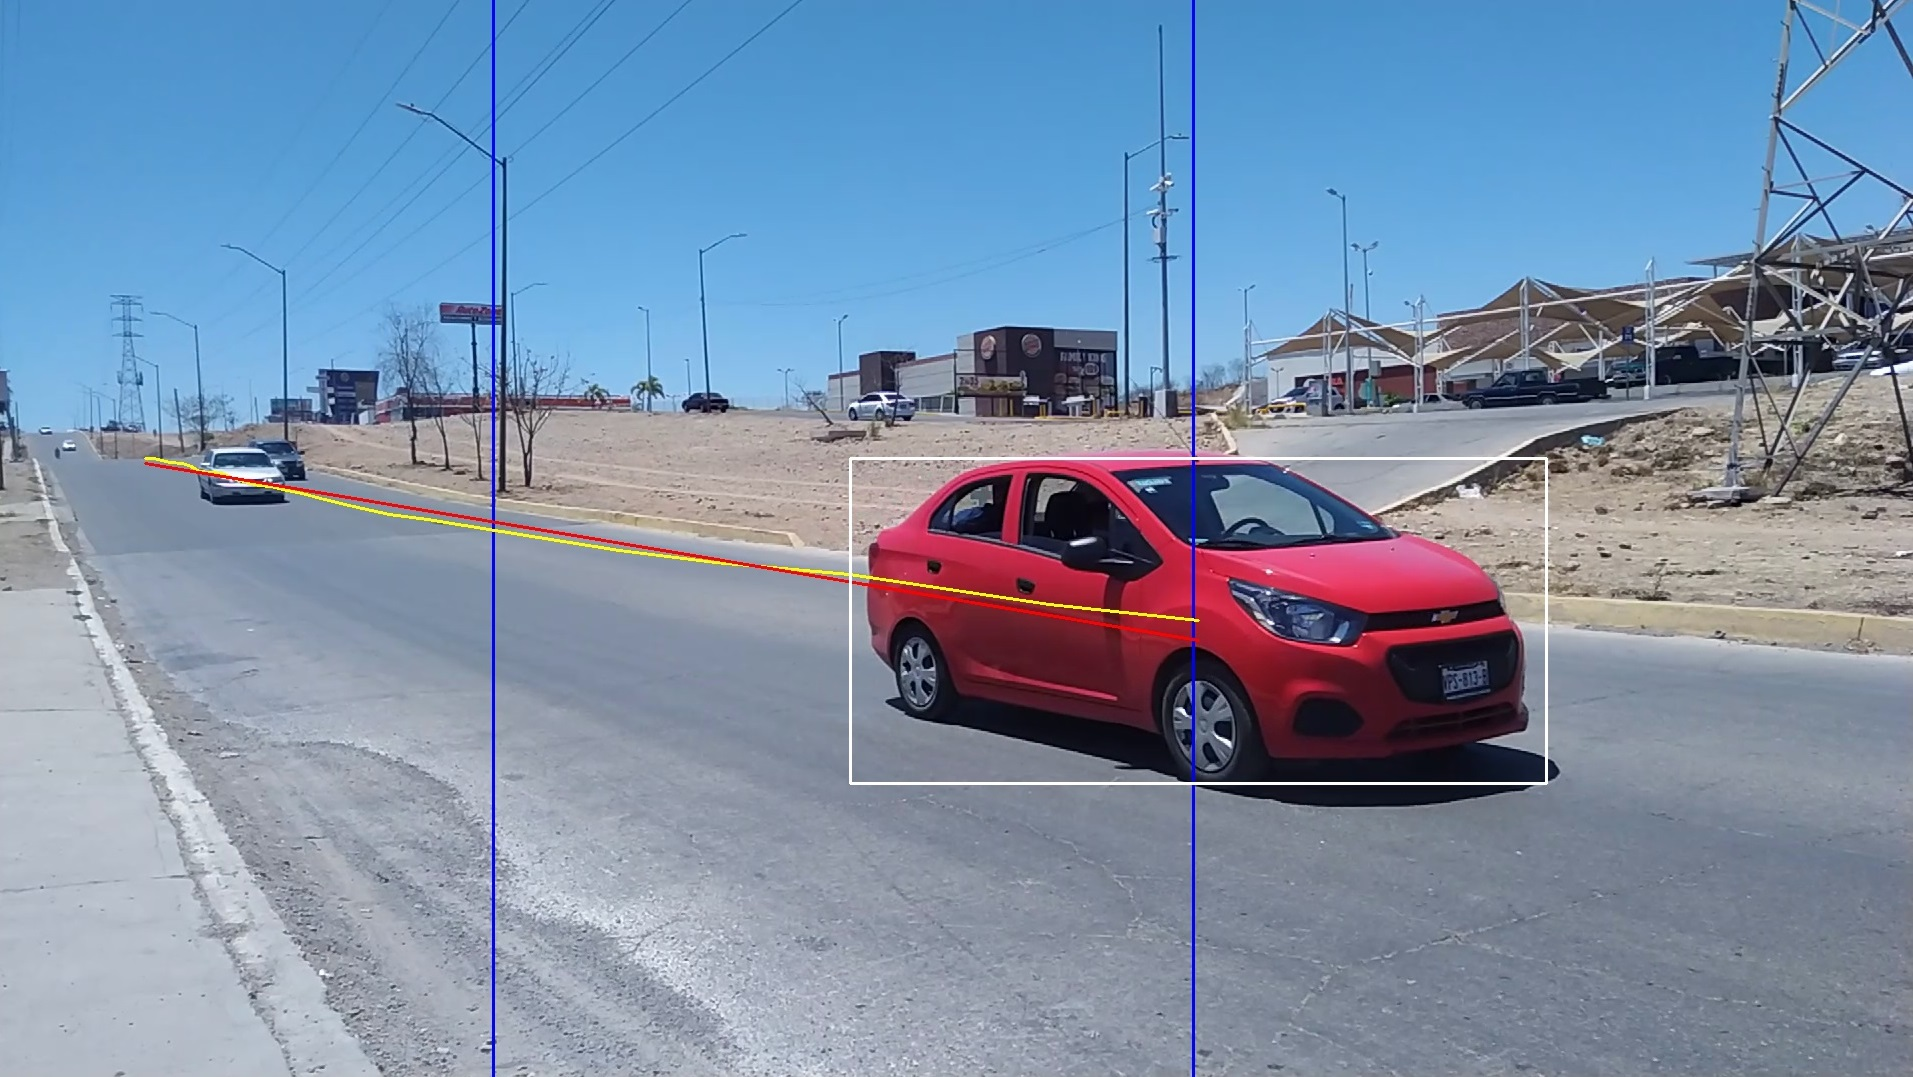
\includegraphics[width=0.4\textwidth]{imgs/track.jpg}
    \centering
    \caption{Vehículo identificado con su respectivo seguimiento.}
    \label{img:Tracking}
\end{figure}
Cuando se detecta que un vehículo pasa por el primer limite se guarda el fotograma para después unirlo con el fotograma pasando por el punto de salida, cabe mencionar que esto se realiza para todos los vehículos detectados. Sin embargo, solo se guardan aquellos que correspondan al segundo de salida que se identificó en el archivo CSV. Una vez se detecta que un vehículo sale del límite, se guardan los datos y la velocidad en una línea del archivo CSV, al mismo tiempo se guarda una imagen con el vehículo entrando y saliendo por los límites, y un identificador para la imagen.
\item \textit{Limpieza de los datos.} El sistema genera una imagen por cada línea del CSV resultante, esta imagen es la combinación de 2 imágenes, cuando el vehículo pasa por el punto de entrada y cuando pasa por el punto de salida, con ayuda de esta imagen validamos que el vehículo haya sido tomado correctamente. Una imagen valida es aquella que no se aleja demasiado del punto de salida y el vehículo se detecta completo o gran parte del mismo.
Para las imágenes invalidas tenemos un vehículo incompleto. La Figura \ref{img:invalid} muestra un ejemplo de un vehículo capturado parcialmente.
\begin{figure}[H]
    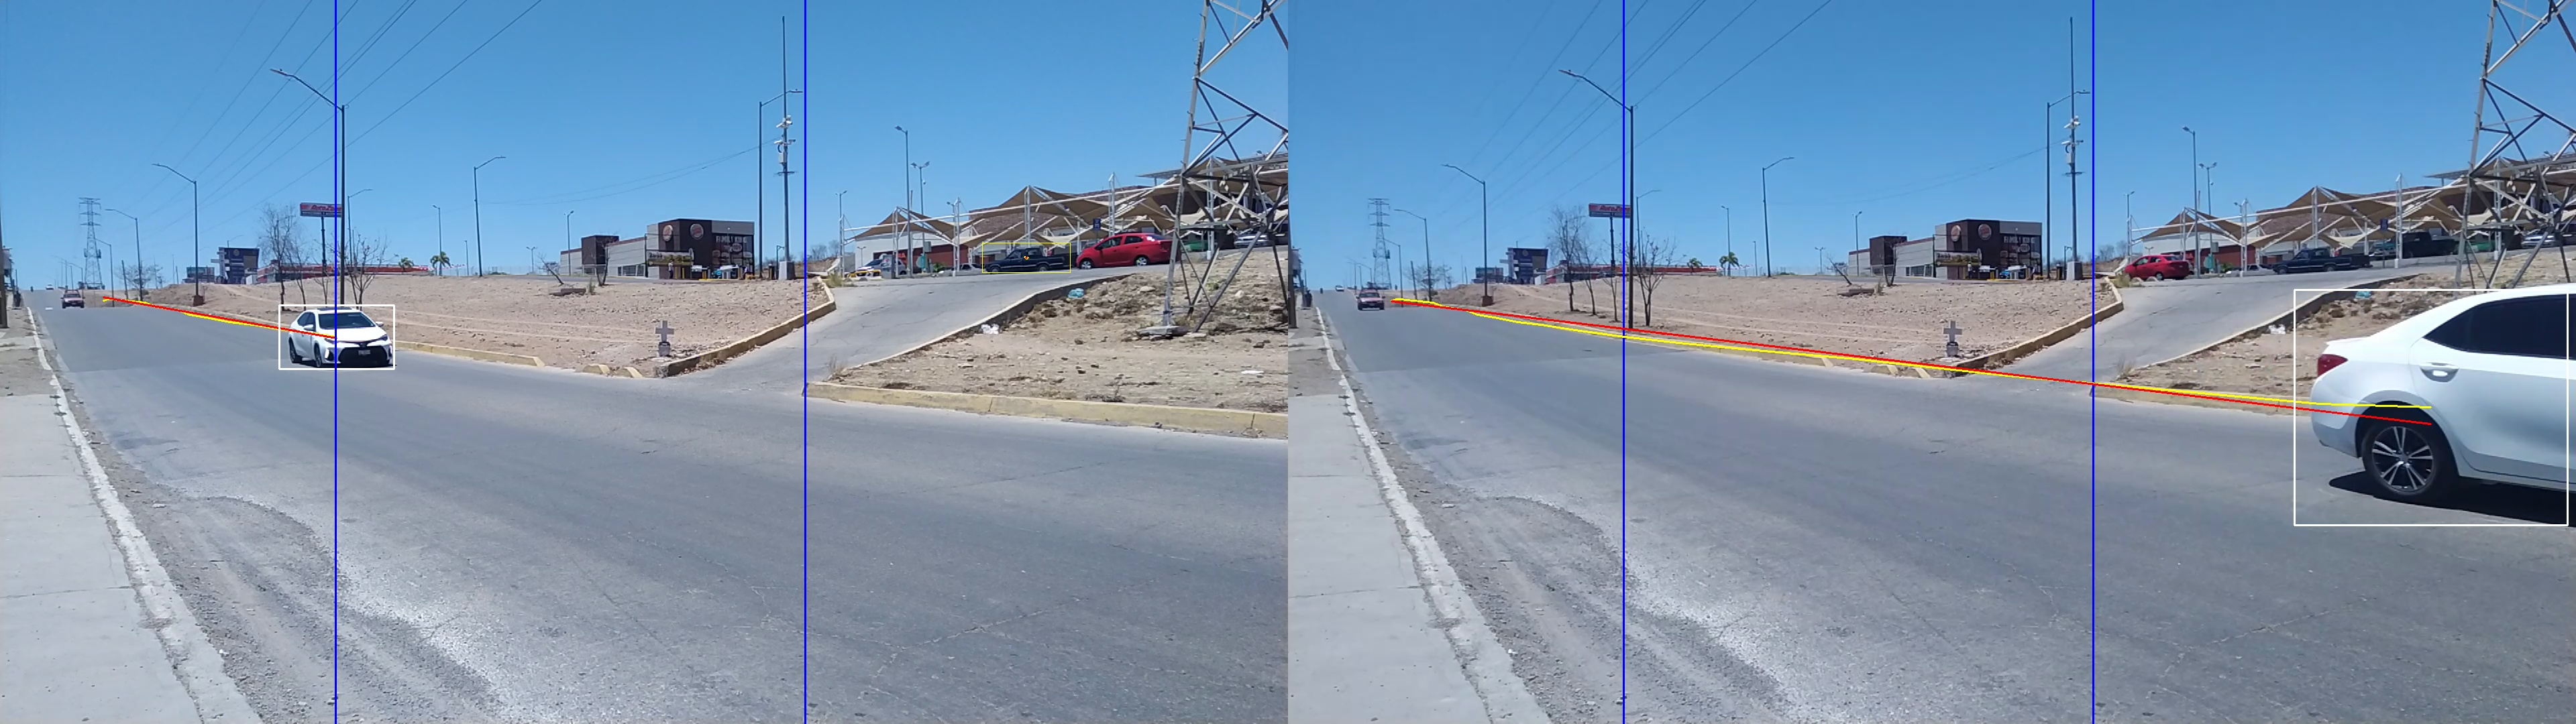
\includegraphics[width=0.65\textwidth]{imgs/img_no_valid.jpg}
    \centering
    \caption{Detección invalida del sistema.}
    \label{img:invalid}
\end{figure}
\end{itemize}
\section{Avances}

Hasta el momento de redactar este articulo contamos con un total de 97 vídeos de entre 1 y 2 minutos de duración, de los cuales solo 51 vídeos han sido procesados. Para finalmente obtener 408 muestras. Ejemplo del resultado obtenido es la Tabla \ref{tab:csv_result} que muestra 3 muestras obtenidas durante el proceso de extracción de características. 

\begin{table} [h]
\caption{Ejemplo de muestras resultantes.}
\label{tab:csv_result}
\centering
\begin{tabular}{|c|c|c|c|c|c|c|c|} 
\hline
\begin{tabular}[c]{@{}c@{}}\textbf{Angulo}\\\textbf{Salida~}\end{tabular} & \begin{tabular}[c]{@{}c@{}}\textbf{Distancia}\\\textbf{Salida~}\end{tabular} & \begin{tabular}[c]{@{}c@{}}\textbf{Area}\\\textbf{Entrada~}\end{tabular} & \begin{tabular}[c]{@{}c@{}}\textbf{Area}\\\textbf{Salida~}\end{tabular} & \textbf{FPS~} & \textbf{Tiempo~} & \textbf{Velocidad~} & \textbf{Identificador~}  \\ 
\hline
78.65~ & 711~ & 26335~ & 145475~ & 60.01~ & 0.866~ & 37~ & 117~ \\ 
\hline
82.71~ & 693~ & 23421~ & 122661~ & 60.01~ & 0.866~ & 32~ & 358~ \\ 
\hline
78.97~ & 700~ & 55815~ & 350730~ & 60.01~ & 0.633~ & 45~ & 407~ \\
\hline
\end{tabular}
\end{table}

La Figura \ref{img:img_result} muestra en un recuadro blanco el vehículo que el sistema esta realizando el seguimiento para generar su información, mientras que en amarillo el resto de los vehículos detectados a los que no se les generara una linea para el CSV resultante.

\begin{figure}[h]
    
    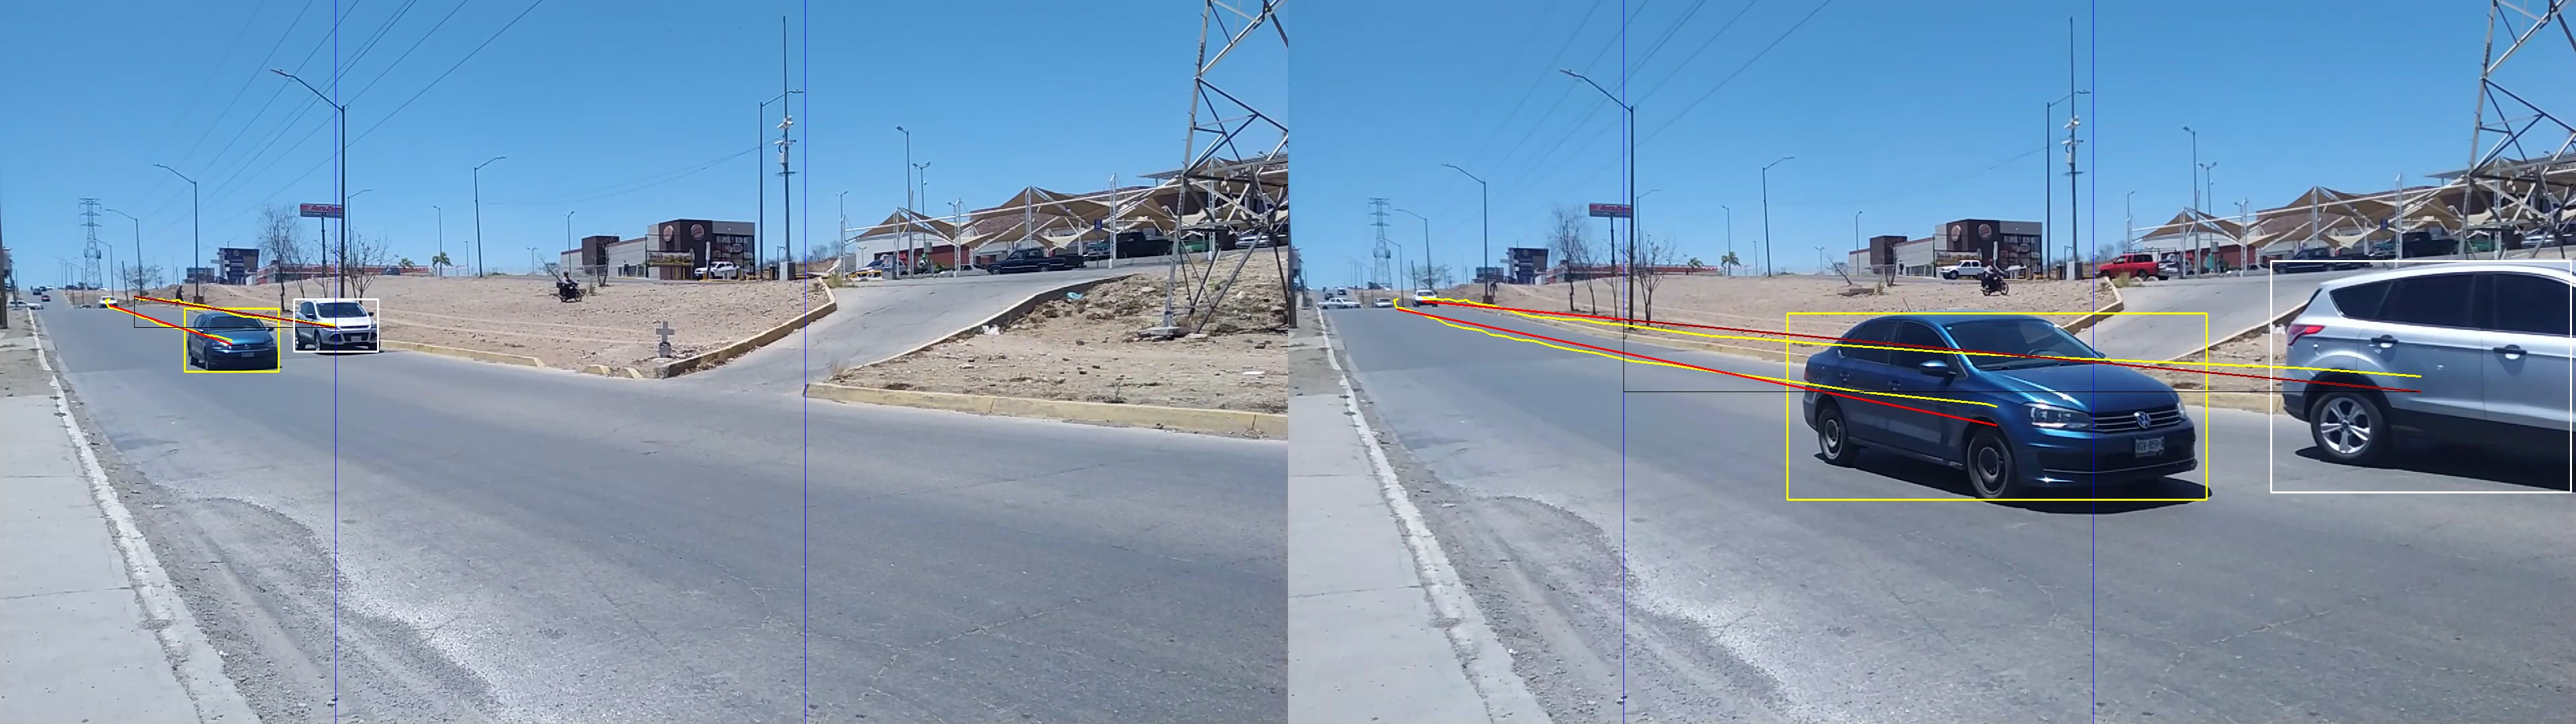
\includegraphics[width=0.65\textwidth]{imgs/img_result.jpg}
    \centering
    \caption{Imagen generada por el sistema.}
    \label{img:img_result}
\end{figure}


\section{Conclusiones}
El sistema es capaz de generar un conjunto de datos de calidad, con este podemos realizar experimentos con diferentes métodos ya sean estadísticos o de inteligencia artificial para predecir la velocidad de objetos que aparecen en una secuencia de vídeo. Además de darnos la libertad de integrar sensores para generar más parámetros que pueden ser de valor para inferir la velocidad de objetos. Por otra parte, el conjunto de datos generado requiere la eliminación de datos que puedan afectar las predicciones, lo cual implica un trabajo extra por parte de quien genera el conjunto de datos, además de tomar una suma considerable de vídeos para generar un conjunto de datos aceptable. Una actividad de mejora importante para el sistema es eliminar la necesidad de una persona que genere el archivo CSV con las velocidades y también quien valida que la información generada es correcta, esto ayudara a reducir el tiempo necesario para generar el conjunto de datos.

%
% ---- Bibliography ----
%
% BibTeX users should specify bibliography style 'splncs04'.
% References will then be sorted and formatted in the correct style.
%
\bibliography{bib.bib}
\bibliographystyle{splncs04}

% \printbibliography

\end{document}
